\section{\bench: Evaluating Agents in a Dual-Control Environment}
\label{sec:methods}

\bench serves as a platform for a systematic study of multi-turn interactions between a conversational AI agent and a simulated user. %
Dual-control interactions are modeled as a Decentralized Partially Observable Markov Decision Process (\decpomdp)~\cite{oliehoek2016concise} where both the agent and user can communicate, use tools, and receive observations. This allows us to simulate complex scenarios like technical troubleshooting where agent and user must coordinate their actions to solve the task.

\subsection{The \decpomdp Formalism}
\label{sec:decpomdp_framework}

As illustrated in \Cref{fig:teaser}, the \decpomdp in \bench involves two players: an agent and a user. The entire process is formally defined by the tuple $(\gS, \{\gA_i\}, \{\gO_i\}, \gT, \gR, \gU, \gM)$, where $i \in \{\agent, \user\}$ denotes players and each component in the tuple is detailed below, with illustrative examples drawn from the new \telecom domain.

\textbf{Message space ($\gM$):} The set of all possible (natural language) messages exchanged between the agent and the user. For example, the user could say ``I cannot use mobile data.'' and the agent could respond with ``Could you check whether your airplane mode is on?''

\textbf{State space ($\gS$):} The global state $\gS = \gS_{world} \otimes \gS_{history}$, where $\gS_{world} = \gS_{db,\agent} \otimes \gS_{db,\user}$ represents the \textit{underlying} database states for the agent and user, and $\gS_{history}$ logs all interaction events (actions, observations, messages). For example, in the \telecom domain, $\gS_{db,\agent}$ might be CRM data (customer profiles, lines), while $\gS_{db,\user}$ could be phone status.

\textbf{Action spaces ($\gA_i$):} Player $i$'s action $a_i \in \gA_i$ is either a tool call $a_{i,tool} \in \gA_{i,tool}$ (interacting with $\gS_{db,i}$ via function calls like \texttt{tool\_name(**kwargs)}) or a message $m_i \in \gM$. Only one player acts per turn. In the \telecom domain, the agent can access tools like \texttt{get\_customer\_by\_id(id)} and the user can access tools like \texttt{toggle\_airplane\_mode()}.

\textbf{Observation spaces ($\gO_i$):} Player $i$'s observation $o_i \in \gO_i$ is either a tool observation $o_{i,tool}$ (e.g., data, messages, or errors from $a_{i,tool}$) or a message $m_j \in \gM$ from player $j \neq i$. Only one player receives an observation per turn. In the \telecom domain, the agent might observe customer details from \texttt{get\_customer\_by\_id}, and the user might observe a message indicating the airplane mode has been turned off from \texttt{toggle\_airplane\_mode}.

\textbf{Transition function ($\gT$):} Defines system dynamics via $\gT: \gS \times \gA \to \gS \times \gO$. Given current state $s \in \gS$ and joint action $a=(a_{\agent}, a_{\user})$, it yields a new state $s' \in \gS$ and joint observation $o = (o_{\agent}, o_{\user})$. Calling a tool $a_{i,tool} \in \gA_{i,tool}$ may change $\gS_{world}$ and yield $o_i \in \gO_{i,tool}$. Sending a message $m_i \in \gM$ yields $o_j=m_i$ for $j \neq i$. In both cases, $s'$ includes updated $\gS_{world}$ and $\gS_{history}$. For example, an agent's action \texttt{enable\_roaming(customer\_id, line\_id)} would update the world state (the roaming service for the specific line number is enabled), and a user's action \texttt{toggle\_airplane\_mode} would update the status of the mocked phone.

\textbf{Reward function ($\gR$):} A function $\gR: \gS \to [0, 1]$ providing a global reward based on the overall state $s \in \gS$ (database states, history), signaling task success or failure. For example, in \telecom, the agent is rewarded if a user's issue ("no mobile data") is fixed, as verified by the user's database state.

\textbf{Instruction space ($\gU$):} The instruction space $\gU$ defines the scenario guiding realistic user simulation, as well as the domain policies to which the agent must adhere when assisting the user.

The Dec-POMDP formalism offers key advantages for simulating complex, interactive scenarios (see \Cref{fig:traj} for an example trajectory of interactions). 
It enables realistic simulation of collaborative environments, such as technical support, where users execute tool actions guided by the agent. This presents agents with crucial coordination and communication challenges. 
Additionally, the formalism enhances user simulation reliability and control; by defining user tools and their effects on the user state, user behavior becomes more predictable and less reliant on extensive natural language prompting.

\begin{figure}[tb]
    \centering
    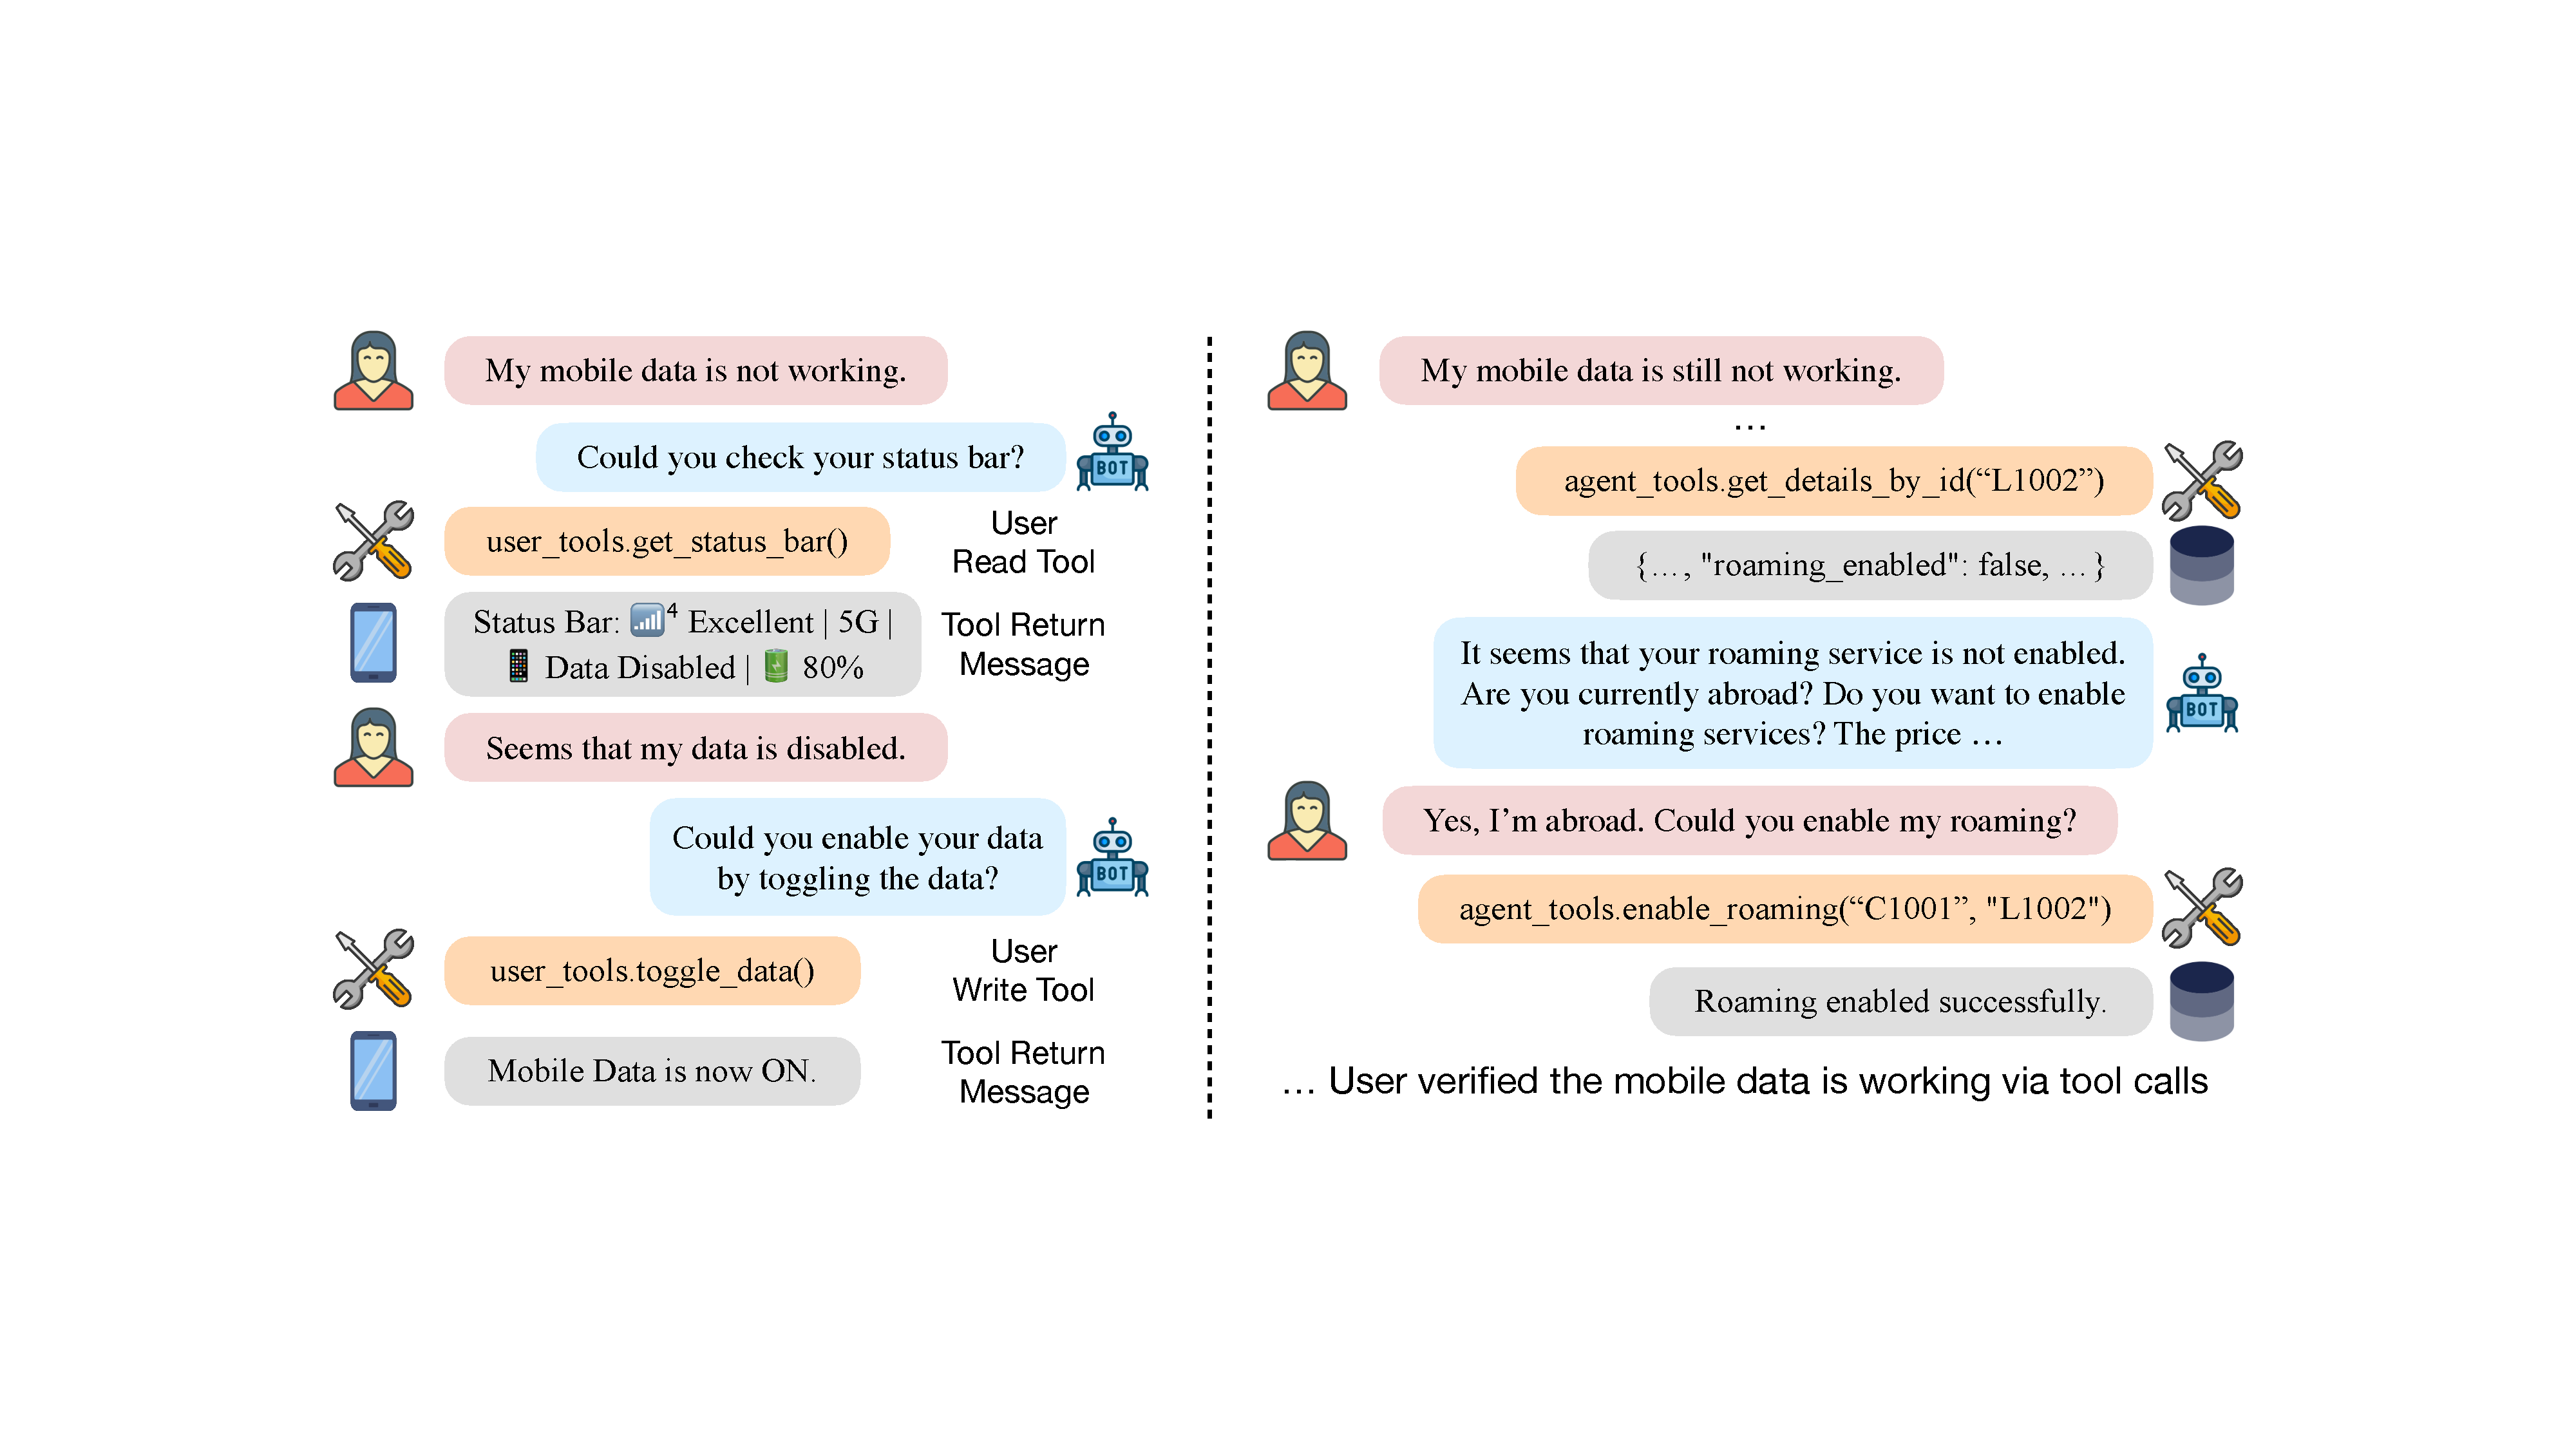
\includegraphics[width=0.99\textwidth,trim=240 240 240 240,clip]{figures/raw/traj.pdf}
    \vspace{-0.5em}
    \caption{An example agent-user interaction trajectory ($\gS_{history}$) of \bench in the \telecom domain. By controlling the implementation of the user tools (the mocked phone), we can reliably simulate the user's response to agent's actionable instructions like ``checking the status bar'' and ``toggling data'' based on the underlying database state. On the right half, we show the possibility of modeling the impact of agent's tool calls on the user's database state, where the roaming service for the user is enabled on the agent's end and therefore allows the user's phone to roam.}
    \label{fig:traj}
\end{figure}


\subsection{Domain and task creation}
\label{sec:curating_domains}

\begin{table}[t]
    \centering
    \caption{Key statistics for the \bench domains.}
    \label{tab:domains}
    \vspace{0.2em}
    \begin{adjustbox}{width=0.95\textwidth}
    \begin{tabular}{llll}
    \toprule
     & \textbf{\retail{}} & \textbf{\airline{}} & \textbf{\telecom{}} \\
    \midrule 
    \textbf{Agent Databases} & 500 users, 50 products, 1,000 orders & 500 users, 300 flights, 2,000 reservations & 5 plans, 9 lines, 4 customers \\
    \textbf{Agent Tools} & 7 write, 6 read & 6 write, 6 read & 6 write, 7 read \\
    \textbf{User Tools} & - & - & 15 write, 15 read \\
    \textbf{Tasks} & 115 & 50 & 114 (full: 2285)\\
    \bottomrule
    \end{tabular}
    \end{adjustbox}
\end{table}


Similar to \taubench, we adopted a multi-stage creation process to build domain-specific materials for new domains. This process, illustrated using the \telecom domain, involves the following stages:

\textbf{Stage 1: Creating agent's database schema and tools.}
We begin by prompting Large Language Models (LLMs) to generate a Product Requirements Document (PRD) that outlines the domain's core business logic. This PRD specifies the database schema and necessary functions. In the \telecom domain, this involved defining a customer CRM system with schemas for customers and lines, along with functions to manage them. An LLM then generates function implementations, a mock database, and unit tests based on the PRD. We manually refine the generated code until all unit tests pass.

\textbf{Stage 2: Creating user's database schema and tools.}
For troubleshooting scenarios, we similarly use an LLM to define the user's database schema and tools. In the \telecom domain, this included implementing a mocked user phone device with status (e.g., signal strength) and functions (e.g., toggling airplane mode). Again, an LLM generates implementations, a mock database, and unit tests, which are then manually refined until all tests pass.

\textbf{Stage 3: Programmatic task creation.}
We employ a combinatorial approach to generate diverse, verifiable tasks from atomic building blocks.

Each atomic subtask $t$ is about a specific problem to be resolved, for example, airplane mode on leads to mobile data not working. Specifically, each subtask $t$ is defined as $(\{f_{t,k}^{init}\}, \{f_{t,k}^{sol}\}, \{f_{t,k}^{assert}\})$, where $f_{t,k}$ is the $k$-th function call of the subtask $t$ that interacts with the agent's or user's database:
\begin{itemize}
    \setlength\itemsep{0em}
    \item \textbf{Initialization functions $f_{t,k}^{init}$} specify calls to set up the initial task state, typically by updating the database values. For instance, in \telecom, an initialization might be \texttt{set\_airplane\_mode(True)}.
    \item \textbf{Solution functions $f_{t,k}^{sol}$} specify tool calls to resolve issues introduced by initialization. For example, \texttt{toggle\_airplane\_mode()} could be a solution for the initialization example given above. Note that these must be tools available to the agent or user.
    \item \textbf{Assertion functions $f_{t,k}^{assert}$} specify conditions the final state $\gS$ must meet for the task to be considered solved. For instance, \texttt{assert\_service\_status("connected")} checks if the user's service is active in \telecom.
\end{itemize}

While solution functions $f_{t,k}^{sol}$ are restricted to agent or user tools, initialization and assertion functions can be any function in the relevant database.

Atomic subtasks are grouped such that mutually exclusive or alternative subtasks are in the same group. A composite task is created by selecting at most one subtask from each group, concatenating their respective function calls.
Task correctness is automatically verified by checking if the final state $s \in \gS$ satisfies all assertion functions after applying initialization and then solution functions. We also verify that the task is not resolved until all solution functions are applied.

In the \telecom domain, we developed 15 atomic subtask groups for 3 user intents of increasing complexity: \serviceissue, \mobiledataissue, and \mmsissue.
Combining these subtasks in a programatic way yields 2285 tasks. We then subsample 114 tasks to form a balanced distribution over different intents and numbers of subtasks (details in \Cref{app:telecom}). The number of subtasks in a task serves as a proxy for difficulty as more diagnostic and resolution steps are required.


\textbf{Stage 4: Creating domain-specific agent policy.}
Based on the curated tasks and their solutions, we prompt LLMs to generate domain-specific policies for the agent. For troubleshooting, these policies guide the agent in diagnosing and resolving user issues, often outlining step-by-step procedures for common problems related to each user intent, details in \Cref{app:telecom-policy}.

\textbf{Stage 5: Manual refinement.} We jointly refine all the domain materials including tools, policy and atomic subtasks to improve the quality of the domain.

Moreover, compared to the original \taubench, \bench enables a developer to specifically associate a task with a Persona (a brief description of the user's identity).
We put this to use in our new domain. Each \telecom domain task was randomly assigned one of the following personas: \texttt{None}, \texttt{Easy}, and \texttt{Hard}. The \texttt{None} persona means that no specific persona is provided to the user simulator. The \texttt{Easy} persona describe the profile of a user who is rather familiar with the domain while the \texttt{Hard} persona represents a more challenging user with low technical knowledge (see \Cref{app:telecom-user-persona}).

\subsection{Task evaluation}
The success of a task can be defined by different criteria: DB check, status assertions, natural language assertions, communication info check, and action matching.
The DB check and communication info check are the same as the original \taubench. The status assertion involves verifying specific conditions in the final world state $\gS_{world}$ using the predefined assertion functions (e.g., checking if a service is connected). The natural language assertion involves verifying specific conditions in the final history state $\gS_{history}$ using a natural language description, like ``the agent diagnosed the cause of the issue.'' The action matching involves verifying if every solution function $f_{t,k}^{sol}$ exists in the actual agent-user interaction trajectory.
Practically, each task can specify a subset of these criteria based on its features. In \telecom, only assertion functions are used to evaluate task success.



